\chapter{Background} \label{Background}

\section{The Need for Explainable AI}

To define the problem that needs to be address, a thorough literature review has been undertaken to fully expose and understand the capabilities and limitations facing the relatively new field of XAI. This requires a broad approach, considering insights from multiple academic fields beyond that of computer science, incorporating findings from the fields of psychology, sociology, philosophy, law, and politics. These investigations ultimately underpin the reasoning behind this project:

\begin{enumerate}
    \item The need for explainable AI: 
        \begin{enumerate}
        \item Dampen alarm amongst all sectors and demographics of digitalised societies
        \item To fulfil existing and proposed legislative requirements
        \item A bulwark to societal risks through the reparation of trust and enabling of accountability
        \item To enable the productive and positive use of AI for all; acknowledging domain context, end users needs and cognitive ability
        \end{enumerate}
    \item How should one define explainability and interpretability? The ubiquitous interchangeable use of terminology by researchers and practitioners e.g. transparency, interpretability, and comprehensibility, often used interchangeably 
    \item The importance of interdisciplinary collaboration and empirical evidence. This requirement needs to be fulfilled to its fullest to demonstrate the validity of the XAI research and/or development e.g. Example through the rigorous use of psychological analytical methods. I comment that one such field ripe for interdisciplinary knowledge sharing, is field of categorisation theory, amongst others such as human factors/ergonomics. XAI algorithm researchers and developers must consider the ways in which the human brain works, with many of the tasks proposed to be solved by AI previously have been done by humans, and if not solved, then used as an assistive tool, of which humans need to be able to interpret.
    \item A critical analysis of the most relevant, prominently used and cutting edge XAI methods. This dissection of the research attempts to inform the design of this research project, with a pronounced focus on that of “Concept Bottleneck Networks” (CBMs) and “Convolutional Neural Networks” (CNNs). The intended goal with these methods is to accurately expose inherently interpretable image features/concepts that can be used as by humans to aid with comprehending a models decision/category classification. A broad analysis is undertaken, looking at two broad strands of methodology inherently interpretable and post-hoc models: the problems pertain to solve, their sufficiency in providing the desired level explainability to their intended users, how the underlying algorithms work and the limitations they face: by design, dataset, lack of domain knowledge, or empirical evidence garnered through experimentation.
\end{enumerate}

The desire for explainability (transparency, understandability, comprehensibility, interpretability etc.) in automation is not a new field, however with the increased opacity of AI decision making and their use by all walks of life (knowingly or not), new methods are required to be able to hold to account, trust and ultimately adopt these new technologies. The term Explainable AI (XAI) was only officially defined in 2017 in a report for the United States of America’s “Defence Advanced Research Projects Agency” (DARPA) \cite{gunningExplainableArtificialIntelligence2017}:

\emph{“XAI will create a suite of machine learning techniques that enables human users to understand, appropriately trust, and effectively manage the emerging generation of artificially intelligent partners”.}

\vspace{1cm}

\subsection{Dampening alarm}

The voracious pace at which Artificial Intelligence (AI) technologies continue to be developed, has raised alarm amongst experts, academics, and society at large, with little recourse to hold its resultant outputs to account. Examples of this include “Correctional Offender Management Profiling for Alternative Sanctions” (COMPAS) system used in the USA to predict a criminal defendant’s likelihood of being repeat offender, of which those in the criminal justice system have become increasingly dependent on. Data analysis as shown that COMPAS makes multiple errors in classification, with an overt inclination to racially profile and mis-classify black defendants as being a higher risk of becoming recidivists compared to their white counterparts \cite{larsonHowWeAnalyzed2016}. The COMPAS algorithm lacks in delivering a clear explanation for its classification, and concurrently due to its secrecy, lacks any form of transparency, removing the opportunity for scrutiny and a sense of procedural fairness for both the defendant and the public \cite{rudinAgeSecrecyUnfairness2020}. The societal use and trust in the technology is convoluted; polarising many due to a lack of an inclusive and transparent sharing of knowledge and information, with many individuals relying solely on information extrapolated from their AI curated media “bubble”, television channel or newspaper, often misinterpreting or overstating the truth for the purpose of supporting their own goals - ones attention, clicks (likes, sharing etc.), advertising or supporting a political agenda.

The development AI tools, thus far has been lead by "practitioners, disproportionately white, male, and advantaged" \cite{lazarAISafetyWhose2023}, creating a perception akin to that of a mono-culture. This lack of ideological and demographic diversity is particularly worrying if harms to society are to be effectively mitigated.

Most recent concerns observed globally have been surrounding the increased application of Generative AI in an ever-expanding set of domains. Deepfakes have arisen in a variety of contexts, from images and videos of actions that have never taken place, to the cloning of voices (\cite{ElevenLabsGenerativeAI}, \cite{SpeechifyCompleteAI2022}) for the criminal manipulation of others, resulting in the divulgence of personal or classified information, often with the intent to obtain money (\cite{federaltradecommissionconsumeradviceScammersUseAI2023}, \cite{pashentsevPalgraveHandbookMalicious2023}). Despite instances such as these clearly supporting a negative perception of voice cloning AI in the public psyche, there are also tremendous benefits. Take for example, a minor instance of a radio or podcast interviewee, who, with consent, will not have to return to the studio to re-record a mispronunciation or incorrect statistic, and in turn potentially saves considerable carbon emissions as a result of travel, as well as a host of peoples time and effort. 

At the extreme end of this spectrum, South Korean president elect \emph{Yoon Suk-Yeol} used a deepfake “AI avatar” in 2022, purportedly helping him to win the younger vote \cite{SouthKoreaPresidential2022}. It’s quite clear to see how this has use of AI has the potential for misuse, misleading people as to the ability or intent of a politician or influenced by nefarious actors out of sight. One such occurrence happened in June 2022 when the mayors of many European capitals were duped in a video conference by a deep fake avatar of Kyiv’s, Vitali Klitschko \cite{pashentsevPalgraveHandbookMalicious2023}. Other domains include that which copy the style of human artists both visually and audibly e.g. fake cover versions of songs using So-VITS-SVC \cite{SoftVCVITSSinging2023}, synthesising new music in the style of artist with OpenAI’s Jukebox \cite{openaiJukebox2023}, the recreation of damaged artworks \cite{googleKlimtVsKlimt2021}, or mimicking of an artist’s style to create new works using as thought they were alive today using OpenAI’s DALL-E 2 (\cite{DALL}, \cite{evansClimateCrisisPaintings2022}). Perhaps the most prevalent usage has been that of using ChatGPT \cite{ChatGPT} and other such Large Language Models (LLMs), to generate fake text content for the web or to write assessed work for academics and students, despite the clear limits currently present e.g. the propensity to hallucinate false academic references (\cite{alkaissiArtificialHallucinationsChatGPT2023}, \cite{waltersFabricationErrorsBibliographic2023}). The extent to which LLMs should be allowed to be incorporated is hotly debated between both students and academics \cite{attewellExploringRoleGenerative2023}. Despite generative AI not being the subject focus of this research project, the rise in deepfakes has placed an even greater emphasis on the inadequacy and necessity for XAI across all domains, as but one of the many buttresses required to deliver this new technology in a responsible and accountable manner.

\subsection{Legislation}

As AI models increase in their capacity for purportedly accurate decision making, they are often so inherently complex, often referred to as the “black box problem”, that even experts in the field are challenged to comprehend them. This inherent opacity has elevated the demand for greater transparency and comprehensibility due to concerns over increased over reliance, lack of accountability and potential inherent biases within the data used to train AI models. Examples that bring this into light include the European Union’s (EU) General Data Protection Regulations (GDPR) that took effect in 2018,  effectively giving a user the “right to explanation” \cite{goodmanEuropeanUnionRegulations2017a}, with proposed revision and changes discussed in the recent “Study on the impact of artificial intelligence on the infringement and enforcement of copyright and designs” by the European Union Intellectual Property Office \cite{europeanunionintellectualpropertyoffice.StudyImpactArtificial2022}. Moves in this direction could also be seen back in 2016 when Bulgaria paved the way in requiring most government software to be open source \cite{coldeweyBulgariaNowRequires2016}, shortly followed by the creation of a New York Task force to investigate ways in which automated systems can be made more transparent \cite{wiggersNewYorkCity2018}. For without the means from which one can be allowed to the opportunity to trust AI in an intelligible, explainable format, the result will leave the user isolated, eroding trust and hampering adoption and the merits AI can bring to society, particularly in those of a critical nature, such as health and safety. 

\subsection{Societal risks, reparation of trust and enabling of accountability}

I hypothesise that one could extrapolate from research in the domains of both computer science, cognitive psychology, and governing body reports (national and global), that without a legally enforced systems for explanatory AI at all levels, there is a great societal risk of political extremism and unrest due to an erosion in trust, a lack of accountability, and subsequently the human propensity to feel a loss of control over ones surroundings (\cite{vanprooijenInfluenceControlBelief2015}, \cite{vanprooijenWhyEducationPredicts2017}). The spread of fake media, and subsequently a propensity to be vulnerable to belief in conspiracy theories. This was made quite apparent with the abundance of fake news propagated through social media, forums, and alternative news channels during the COVID19 pandemic \cite{apukeFakeNewsCOVID192021}. Zellers et al.'s paper “Defending Against Neural Fake News” \cite{NEURIPS2019_3e9f0fc9}, could not have been timelier, with it's publication in 2019, just prior to the COVID19 pandemic. One of the most interesting points noted in the paper was that human readers were often prone to perceiving machine generated text as more trustworthy than human-written. Many means of automated fact checking have emerged and is well summarised by Guo et al. \cite{guoSurveyAutomatedFactChecking2022}, who notes that not only text processing, but multi-modal (image, audio, and video) forms of fact checking are required, however its limitations will be dependent on large-scale annotated datasets paired with evidence beyond that of metadata being required. Van Prooijen et al. (\cite{vanprooijenInfluenceControlBelief2015}, \cite{vanprooijenWhyEducationPredicts2017}) conducted research into this domain in multiple research papers. In 2015 Van Prooijen et al. conducted two studies in an applied setting, one measuring participants looking into the beliefs about conspiracy theories and public policy, and the other using a data set collected just prior to the year 2000, surveying attitudes to the threat of the Y2K bug, also known as the millennium bug, alongside beliefs in conspiracy theories that were prevalent at the time. The research shows that the “human need for control is closely coupled with their tendency to believe in conspiracy theories”. In 2017 Van Prooijen et al. went further by exploring the question of why education attainment is often used to predict belief in conspiracy theories. The results in the study conclude that there are at least two mediators in this link; that of “cognitive complexity” (analytical thinking vs belief in simple solutions) and “feeling of control” (can citizens influence government, can citizens express their thoughts and feelings about government decisions etc.). 

This analysis, despite being beyond the scope of XAI intended for use by experts, for which this is subject of this dissertation, remains pertinent. For if individuals and/or society are to trust and hold to account expert users of AI, an elucidation, and comprehension of the constraints and limitations of a systems functionality is imperative. This further underlines the need for a positive and transparent dialectic between governments, technology enterprises and the broader society, to disseminate accurate information as to the true capabilities and limitations of AI \cite{worldeconomicforumPresidioRecommendationsResponsible2023}. 

\subsection{AI for all: domain context, user needs and cognitive ability}

A wide variety of users and stakeholders engage with AI tools e.g. virtual assistants, smart speakers and social robots, however many fail to notice their prevalence in broader domains such as facial recognition, digital photo-tagging, and recommendation engines \cite{zhangArtificialIntelligenceAmerican2019}. As such, holding there systems accountable requires a host of different means, depending upon the domain, the user, their needs and cognitive ability (\cite{goodmanEuropeanUnionRegulations2017a},\cite{amarasingheImportanceApplicationGroundedExperimental2023}, \cite{hoffmanEvaluatingMachinegeneratedExplanations2023}, \cite{hoffmanMeasuresExplainableAI2023}, \cite{jesusHowCanChoose2021}, \cite{mohseniMultidisciplinarySurveyFramework2021}, \cite{sovranoExplanatoryArtificialIntelligence2022}, \cite{wangChatCADInteractiveComputerAided2023}, \cite{zhangMayAskFollowup2023}, \cite{danksGovernanceExplainability2022}, \cite{hassijaInterpretingBlackBoxModels2023}, \cite{barredoarrietaExplainableArtificialIntelligence2020}) . In a study comprised of cognitive interviews with senior and mid-career professions \cite{hoffmanExplainableAIRoles2023}, all of whom have experience in AL and/or autonomous systems, and hold post-graduate degrees. Despite his insights being illuminating, they pertain to a limited range of user demographics (18 participants – 16 male, 2 female), showing that an explanation (global or local) is not always needed depending on the role of the individual, their style and circumstance. Trust is a key issue, particularly in the individuals developing the AI tool, with training and troubleshooting being key. However, all those questioned did desire the knowledge that they needed a “satisfactory understating of something, either the AI or the data that was fed to it, at least some of the time. The study underlines the importance of a Human-Computer Interdependence approach to development, whereby the design and evaluation of an AI (and XAI) system, is evaluated in context, including edge cases. The underlying message in this paper is that “individuals prefer to engage in explanation, rather than being passive recipients of explanatory materials” \cite{hoffmanExplainableAIRoles2023}.

Hoffman's research however ignores the prevalence of AI outside of the professional domain. The target audience with which XAI is required is far more diverse, and should be considered the key grounding point from which one should start by first fully understanding, prior to the development of an XAI tool: who is the target audience, and what why do they need it? \cite{barredoarrietaExplainableArtificialIntelligence2020}. This requires knowledge of the user’s cognitive skills, goals, and subsequent ability to understand and comprehend what the XAI tool is showing to them.

\section{How should one define explainability and interpretability?}

The challenges facing the field of XAI concern many researchers, as demonstrable with the veritable increase in papers that undertake the task of surveying and taxonomizing the wide variety of XAI approaches and definitions. Samek et al. \cite{samekExplainableAIInterpreting2019} outline this very point, stating that a “theory of explainable AI, with a formal and universally agreed definition of what explanations are, is lacking”. 

One interpretation of "Interpretability" can be described as a passive characteristic by which a human observer can make sense of a model, a concept that can also be expressed by the term "transparency". Conversely, the term "explainability" should be understood as an active characteristic of a model, clarifying it’s intent as an interface between the user and the decision making process. That is, it endeavours to deliver an accurate proxy of the decision in a format comprehensible to humans \cite{guidottiSurveyMethodsExplaining2019}. 

Barredo Arrieta et al. \cite{barredoarrietaExplainableArtificialIntelligence2020} further contribute to clarification by addressing the multitude of terms frequently used in the field. "Understandability" (or "intelligibility"), should be understood as the ability for one to grasp how a model works, without the need for a full explanation of its structure or algorithmic methods for processing data. "Comprehensibility" (or "interpretability") on the other hand, is akin to the ability of an ML model's ability to present learned knowledge in a format that is inherently interpretable by humans: incorporating both quantitative and qualitative information in an integrated manner. The term "transparency" should be considered primarily when judging the varying degrees of understandabilty (or "intelligibility"): simulatable models, decomposable models and algorithmically transparent models \cite{liptonMythosModelInterpretability2016}.

Mohseni et al. \cite{mohseniMultidisciplinarySurveyFramework2021} propose that common terminology can be broken down under two high-level concepts, "Intelligible Systems" and "Transparent AI" \cite{mohseniMultidisciplinarySurveyFramework2021}, both subsequently comprised of a set of desired properties and desired outcomes (see Table 1 \cite{mohseniMultidisciplinarySurveyFramework2021}). "Interpretable AI", here defined as being a low complexity ML algorithm, and "Explainable AI", defined in a manner not dissimilar to Guidotti et al., are both categorised as practical approaches for implementing "Transparent AI" \cite{mohseniMultidisciplinarySurveyFramework2021}.


\section{The importance of interdisciplinary collaboration and empirical evidence}

It is imperative that that interdisciplinary collaboration and empirical evidence for the validity of XAI developments takes place, and should not be understated.

As AI systems increase to be seamlessly interwoven into our everyday lives, the volume of high quality peer reviewed research required in order to keep abreast of new advancements, both in bare-bones AI (CNNs, LLMs, GAI etc.) and XAI, should be undertaken in a rapacious manner. However, the promises XAI tools make of delivering meaningful and comprehensible explanations are often limited, often due to the singularity of disciplinary insight of the authors. To counter this issue, experts from a diverse range of disciplines should be called upon, from computer science, machine learning (ML), human-computer interactions (HCI), psychology, philosophy, sociology, law, politics and so on \cite{cabitzaQuodEratDemonstrandum2023}.  Diverse perspectives are essential in giving insight on the multifaceted challenges that each academic, and professional domain faces, as well as society as a whole \cite{lazarAISafetyWhose2023}.

Two disciplines that are progressively engaging in collaborative endeavours are, computer science, encompassing areas such as ML and HCI, and psychology (\cite{grangeXAISelfexplanatoryAI2022},\cite{hoffmanEvaluatingMachinegeneratedExplanations2023}). These combined efforts are driving the development of some of the most advanced XAI tools, with the aim of incorporating psychological theories of human cognition, such as categorisation, decision making, and measurements of trust, alongside novel AI algorithms and mixed modalities. Experimental-psychologists are in a unique position, possessing the requisite tools to empirically test XAI systems in experimental settings. Furthermore, ethical domains such as philosophy and sociology are increasingly entering the discourse (\cite{lazarAISafetyWhose2023}, \cite{lazarPowerAINature2022}, \cite{bennWhatWrongAutomated2022}, \cite{zimmermannPoliticalPhilosophyData2022}), providing a crucially needed evaluation of AI legitimacy and safety within the domains it is employed \cite{greeneAIGovernanceMultistakeholder2022}.

Various methods and tools for psychometric analysis and evaluations of AI and XAI have recently been developed, particularly in regards to the concept of trust (\cite{hoffmanMeasuresExplainableAI2023}, \cite{kleinMinimumNecessaryRigor2023}, \cite{hoffmanEvaluatingMachinegeneratedExplanations2023}, \cite{perrigTrustIssuesTrust2023}). The concept of "trust" is intriguing in its ambiguity; a multidimensional factor of on going debate as to its meaning, particularly in the field of Human Factors and Ergonomics. Few AI researchers undertake a considered approach when assessing trust in their work, with many referring to a single definition by Lee and See \cite{leeTrustAutomationDesigning2004a} \cite{uenoTrustHumanAIInteraction2022}.

The most commonly used tool in AI research has been the "Trust between People and Automation" scale (TPA) \cite{jianFoundationsEmpiricallyDetermined2000}, however a more recent metric has been developed with the specific purpose of evaluating XAI, the "Trust Scale for Explainable AI" scale (TXAI) \cite{hoffmanMeasuresExplainableAI2023}. Despite TPA being the most commonly used, the majority of AI studies rely on defining their own questionnaires and definitions of trust, making it almost impossible to validate one AI model against another \cite{uenoTrustHumanAIInteraction2022}. In light of this, TPA and TXAI have been evaluated empirically in the context of AI for the first time through an online study comprised of 1368 participants \cite{perrigTrustIssuesTrust2023}. Results from the study suggest that TXAI (an 8 item questionnaire, using a 5 point Likert-type scale) is most fit for purpose, however the 6th item ("I am wary of the AI") should be removed, leaving no negatively worded items in the scale, preventing misinterpretation by participants and miscoding by researchers alike. These suggestions are congruent with the set of best practices proposed by Schrum et al. \cite{schrumConcerningTrendsLikert2023}, who's research into the use of Likert scales for statistical analysis of human-robot interaction (HRI) experiments, is highly transferable to the domain AI. 

\begin{figure}[H]
  \centering
    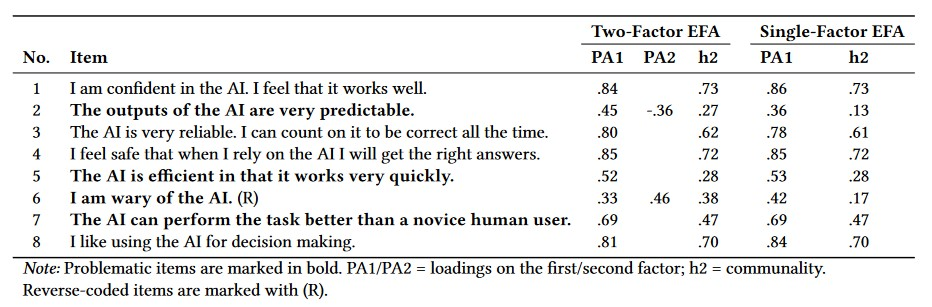
\includegraphics[width=0.8\textwidth]{images/Taken from Perrig et al - Trust tissues with trust scales - review of TXAI by Hofman - 2023.jpg}
  \caption{8 item scale from Hoffman et al \cite{hoffmanMeasuresExplainableAI2023}. As presented in: \cite{perrigTrustIssuesTrust2023}.}\label{fig:CorrectingTXAI}
\end{figure}


Complementary to the assessment of trust, Klein et al. \cite{kleinMinimumNecessaryRigor2023} have set out a framework of 11 requirements by which to guide researchers to run smaller efficient experiments to evaluate human-AI work systems. This new methodology of "Minimum Necessary Rigor" for empirical evaluation of AI is considered necessary in light of the limitations of existing practices which suffer from at the consequence of "rigor mortis": requiring significant funds, large participant pools and complex design and often providing answers no longer required by the time of completion. This method is somewhat contrary to common practice, which promotes the use of a calculating a required sample size for achieving a statistically significant effect on a parametric test \cite{erdfelderGPOWERGeneralPower1996}. This new methodological approach should be being welcomed in light of the voracious pace of AI development, however there is yet any evidence in the literature of its use in practice at time of writing. As such, one should see this proposal as a springboard for discussion, enticing academics to put it into practice and potentially embark on further well scoped, and replicable evaluation methods. Therefore until adequate evidence of its sufficiency is obtained, one should be sceptical until proven otherwise.

In order to build out human centred XAI systems numerous studies and frameworks have been built (\cite{mohseniMultidisciplinarySurveyFramework2021}, \cite{uenoTrustHumanAIInteraction2022},\cite{hoffmanIncreasingValueXAI2023}, \cite{hoffmanMeasuresExplainableAI2023}, \cite{collinsHumanUncertaintyConceptBased2023}) with strong evidence suggesting that feedback modalities with AI systems are key to the their use, with the ability to converse "improving comprehension, acceptance trust and collaboration" \cite{zhangMayAskFollowup2023}. However the use of LLMs as the sole tool for human computer interaction with AI poses significant ethical risks in light of the current lack of XAI methods being deployed \cite{zhaoExplainabilityLargeLanguage2023}.

The fundamental purpose of XAI tools, beyond that of academic research, is that they are intended for practical use in real world domains, in high-stakes decision making, such as medical diagnosis, automated driving, detecting deep-fakes or LLM generated text. This fundamentally requires incorporating the user from inception to deployment. 

High-stakes decision tasks are a prime use case for XAI, yet due to their nature, often problematic to study due to the requirement of developing experiments that are abstracted from the reality.

Examples such as ChatCAD \cite{wangChatCADInteractiveComputerAided2023} demonstrate the possible capabilities in the realm of medical diagnosis and engagement, enabling patients whom may not have access to a doctor the ability to question and garner further insight into their condition. However, ChatCAD has not been discussed nor reviewed by medical practitioners, highlighting the need for far greater interdisciplinary collaboration. 

Leichtmann et al. conducted an exploratory study into the use of XAI \cite{leichtmannEffectsExplainableArtificial2023}, assessing the use of XAI for the high-stake task of deciding if a mushroom is edible or poisonous. The XAI interface delivered an attribution-based example using Grad-CAM \cite{selvarajuGradCAMVisualExplanations2017}, of which the results were statistically significant in improving participants performance in mushroom picking. There are however multiple limitations with this study, such as being restricted to conducting it online rather in the field, and by the sole use of Grad-CAM, of which despite performing better than  LIME \cite{ribeiroWhyShouldTrust2016}, still pertains the intrinsic issues that befall all visual mapping tools.

Alternative XAI methods such as LIME, SHAP, SmoothGrad and Integrated Gradients that are more frequently used have garnered a larger pool of critical research, of which is tackled in the following chapter.

\section{Prior research - the foundation of this project}

To understand the motivations and subsequent approach that this project took, it is necessary for one to grasp the concepts, reasoning, and methodology of the research paper on which it builds upon, along with the limitations therein.

In 2022 Grange et al. \cite{grangeXAISelfexplanatoryAI2022} published a paper presenting a novel methodological approach for constructing an inherently understandable AI. Motivated by the desire to improve AI accountability, increase trust, and adoption, primarily in the high-stakes decision making applications involving health, safety and risk. 

The research approach was primarily grounded in the field of Psychology, drawing upon a body of research conducted by Nosofsky et al. (\cite{sandersTrainingDeepNetworks2020}, \cite{nosofskyTestsExemplarmemoryModel2018}, \cite{miyatsuFeatureHighlightingEnhances2019}) whose expertise and publications in the realm of human categorisation theory had recently highlighted the potential interest of Deep Neural Networks (DNNs) to the field.

Human categorisation theory encompasses various mathematical models, such as mixed representations and rules of the mind(\cite{ashbyNeuropsychologicalTheoryMultiple1998}, \cite{ericksonRulesExemplarsCategory1996}), as well as prototypes \cite{smithThirtyCategorizationResults2000} and exemplars (\cite{nosofskyAttentionSimilarityIdentificationCategorization1986a}, \cite{medinContextTheoryClassification1978}, \cite{kruschkeALCOVEExemplarBasedConnectionist1992}), of which the latter two are grounded upon the notion that categorisation is based upon similarity judgements. Prototype and exemplar model domain research has predominantly been constrained to the use of artificially created categories for systematic assessment and review due to the nature of the complexity of real-world categories. 

Recent advances in DNNs have been employed to predict human similarity judgements \cite{sandersTrainingDeepNetworks2020}, revealing the possibility of shared underlying properties for similarity judgements between AI systems and humans. This subsequently prompted psychologists to further explore the depths of these mutual interpretations. Grange et al. demonstrated this explicitly through a partially feature constrained model, which exhibited a strong correlation with the 8 feature dimensions identified by Nosofsky et al. \cite{miyatsuFeatureHighlightingEnhances2019} and the resultant multi-dimensional scaling (MDS) co-ordinates \cite{sandersTrainingDeepNetworks2020}.

\begin{figure}[H]
  \centering
    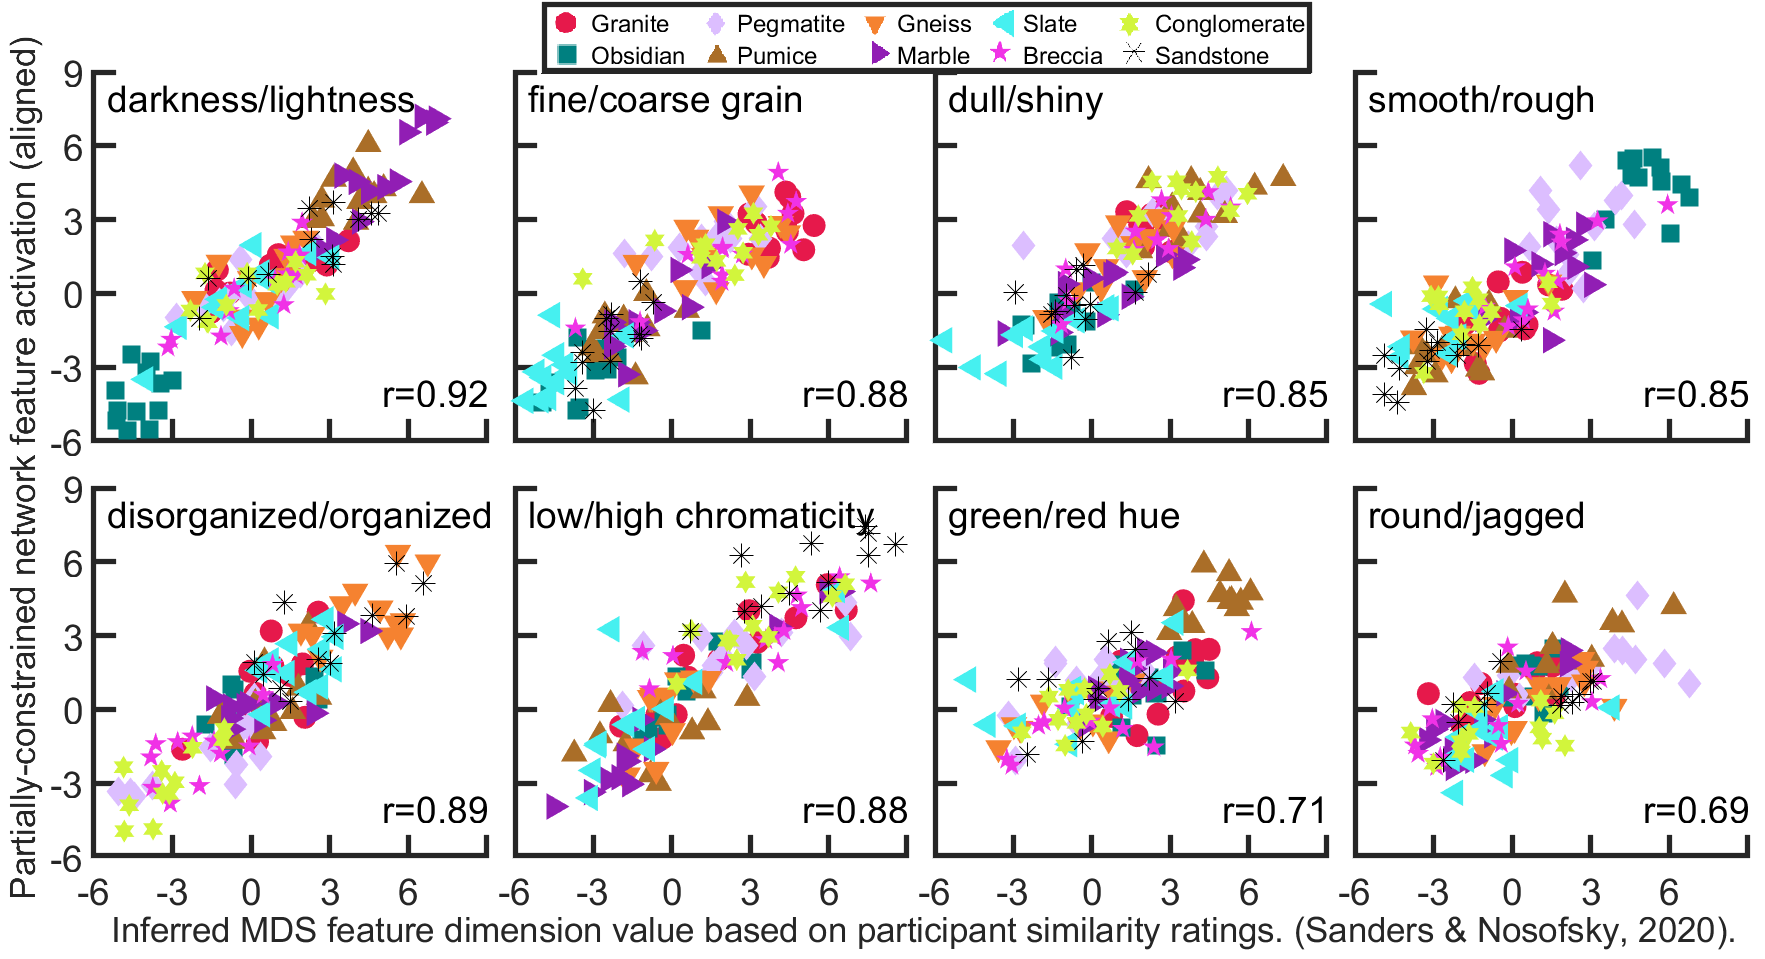
\includegraphics[width=0.8\textwidth]{images/KES2022- MDSvsNetwork Final.PNG}
  \caption{Abstracted features are found to be an affine transform of the Sanders and Nosofsky (2020) inferred MDS feature dimension values based on naïve participants’ similarity ratings. Each plot specifies the MDS feature dimension and the Pearson’s r correlation coefficient. As presented in: \cite{grangeXAISelfexplanatoryAI2022}.}\label{fig:AffineTransform}
\end{figure}

A prerequisite of any explainable and intelligible AI system is the establishment of a shared understanding of concepts. Humans, in general, are less adept at articulating their motivations for categorisation due to complex reasoning, lacking a formal basis on which to do so. On the contrary, domain experts are often intrinsically more adept to do so, equipped with knowledge needed to establish a basis for more profound comprehension of shared concepts between AI systems and experts.

Grange et al. chose the domain of rock classification primarily due to the availability of Nosofsky et al.'s real-world labelled dataset of images and concept/feature ratings, with assessed similarity properties. The similarity judgements from naïve participants enabled the collation of a large database of MDS co-ordinates, from which to input to a low-dimensional similarity space. Due to the high cost of building such a database, Nosofsky et al. circumvented the need to acquire further similarity ratings for new category instances by developing a DNN that successfully predicted MDS co-ordinates \cite{sandersTrainingDeepNetworks2020}.

It's worthy of note that the presence of expert-identified features, from which naïve participants made similarity judgements, expedited participants natural category learning \cite{miyatsuFeatureHighlightingEnhances2019}. As such, further motivating the use of this domain and dataset from which to develop an inherently understandable AI. 

Despite the impressive quality of the ratings data, the collection of rock images was limited in scale when compared to those used to train other AI models e.g. CUB \cite{wahCaltechUCSDBirds2002011Dataset2011}, which comprises of \emph{n} = 11,788 bird photographs. Nosofsky et al.'s set of rock images used in this paper significantly restricted, with 160 "full size" per rock category (n = 1,600), of which 320 random patches were generated and subsequently augmented (translated, flipped, rotated and scaled) to create a set of 480 (n = 4,800).

Thorough employing transfer learning, the penultimate layer of 2048 node activation's (referred to as the "Average Pooling Layer") were  utilised as input into a neural network. These activation's, denoted as  "X train", were combined with a dataset of manually annotated expert feature concepts (Y train), to train the network to predict equivalent expert features. These constrained predicted-feature concepts were subsequently utilised as training data for a single-layer classifier. The fully feature constrained network performed well, achieving a classification accuracy mean of 85.1\% (SD 0.7\%), only 1.7\% short of an unconstrained network’s accuracy mean of 86.8\% (SD 0.8\%).

\begin{figure}[H]
  \centering
    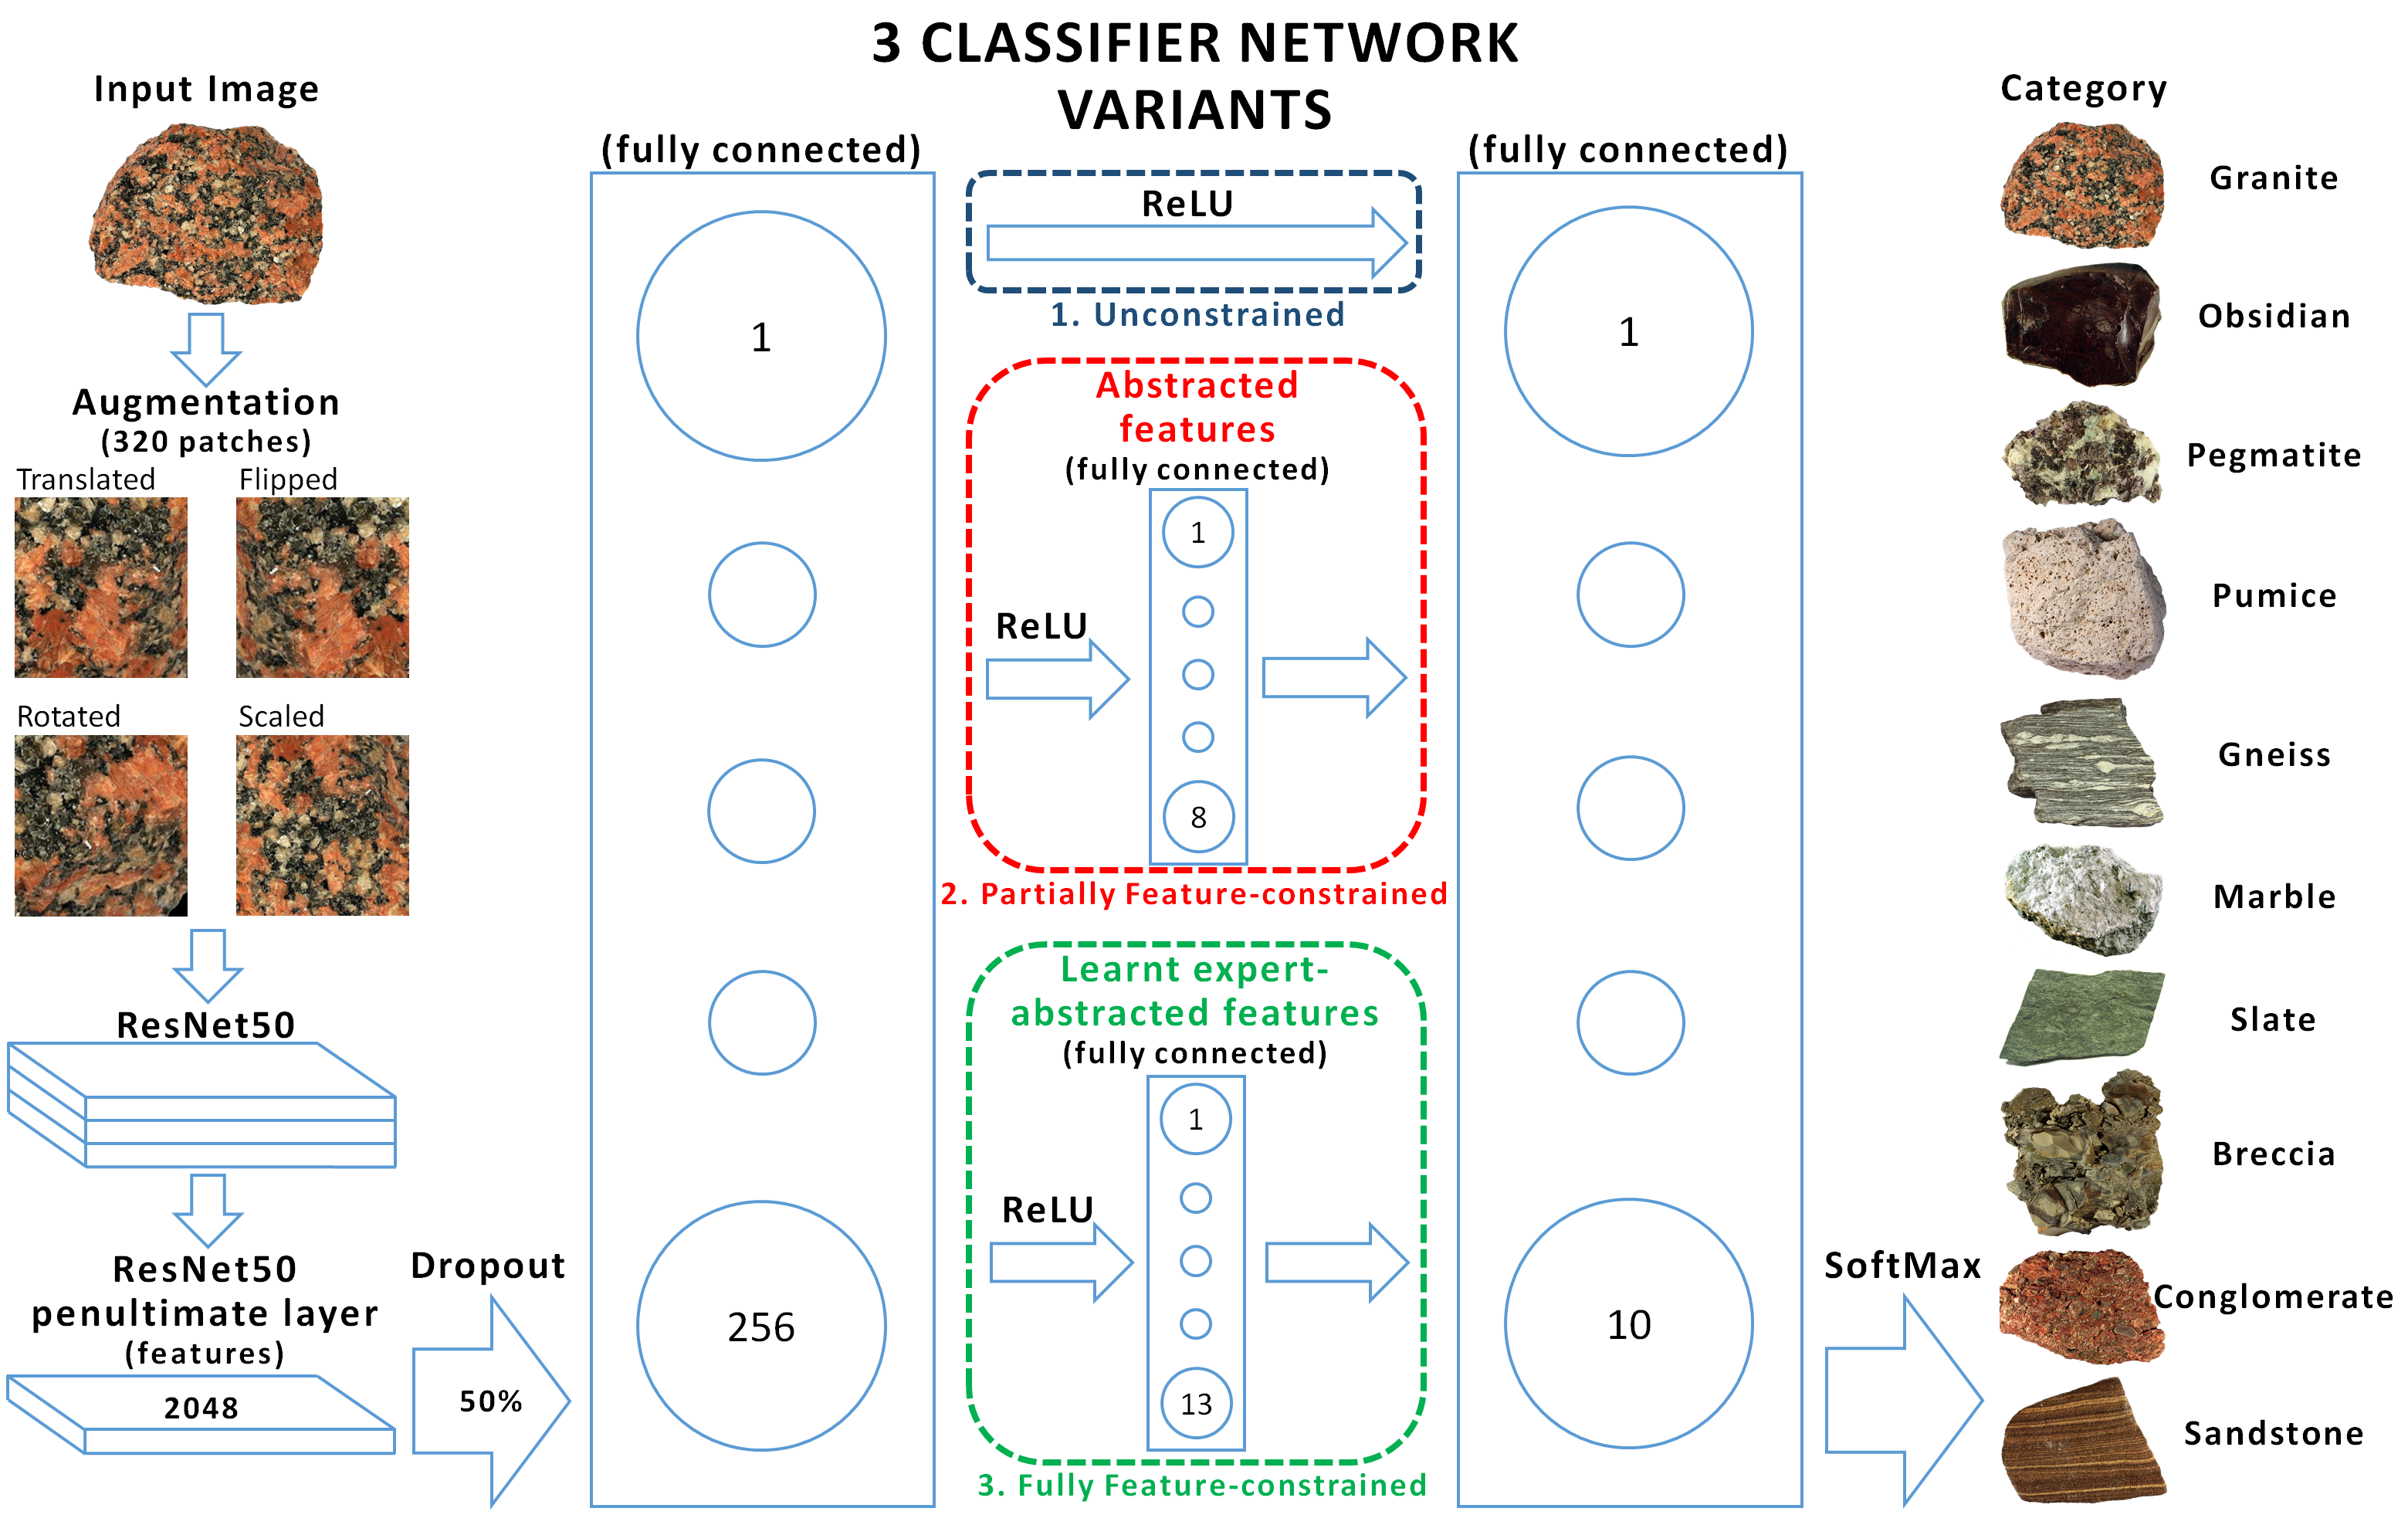
\includegraphics[width=\textwidth]{images/Figure1 - Networks 1-3.png}
    \caption{Illustration of the three classifier network variants making use of transfer learning with Renset50. Rock images are first augmented before being fed through Resnet50, the penultimate layer of Resnet50 is taken through a 50\% drop-out layer, a fully connected 256-node layer, then one of three paths before a 10-node category activation layer is passed through a SoftMax function: (1) an unconstrained variant path, where the 256 node layer fully connects to the 10-node layer through a ReLU function, (2) a partially feature-constrained variant path, where the 256-node layer activations are condensed, via a ReLU function, down to an 8-node, ‘Abstracted Features’ layer and (3) a fully feature-constrained variant path, where the abstracted feature layer is forced to be made of transfer-learned expert-abstracted features. As presented in: \cite{grangeXAISelfexplanatoryAI2022}.}\label{fig:Networks 1-3 XAI&I}
\end{figure}

The finding that an accuracy mean accuracy gap of only 1.7\% between that of the constrained and unconstrained black-box model is impressive. There is however a lack of analysis of features, assessing if any may overlap in knowledge representation, particularly when the correlation between the expert feature ratings and the predicted feature ratings is below that of those which highly correlate e.g. “Brightness Heterogeneity” (r=0.43) compared to “Roughness” (r=0.92).  Further review is also required to understand the nature of features that are rated in a continuous scalar fashion (soft coded) i.e. “Average Grainsize”, compared to that of those with binary ratings (hard coded) e.g. “Presence of Crystals”. A considerable body of research in similar methods shall be critiqued in this dissertation, in support of both binary and scalar methods of coding concepts. 

This begs the question of whether DNNs are interpreting non-binary concept/feature ratings beyond binary distinctions, as many of the features in this model lean towards continuous ratings. However, one should consider if the DNN is perceiving features that are visible in the image or features that are intrinsic to the category/classification type. For example, “Granite” always contains crystals, yet the extent to which they are present may not be equally visible from every image angle.

\section{A Review of Relevant and Recent XAI Methods}

As XAI developers and researchers alike strive to develop new insight and tools with the aim of delivering improvements on the interpretability and explainability of models for a wide variety of users, there ultimately lies a distinction between which route they choose to take to deliver on these promises. This varies dramatically based upon the domain scope (local or global), stage (ante-hoc or post-hoc) and the output format (numerical, visual, textual or mixed) \cite{yangSurveyExplainableAI2023}.

Chen at al. \cite{chenConceptWhiteningInterpretable2020} propose defining interpretability and explainability methods based upon stage alone:
\begin{enumerate}
    \item Ante-hoc, inherently interpretable models (\cite{chenConceptWhiteningInterpretable2020}, \cite{kohConceptBottleneckModels2020}, \cite{havasiAddressingLeakageConcept2022a}, \cite{rudinInterpretableMachineLearning2021}, \cite{eltonSelfexplainingAIAlternative2020}, \cite{grangeXAISelfexplanatoryAI2022})
    \item Post-hoc explanations for existing neural networks (\cite{ribeiroWhyShouldTrust2016}, \cite{lundbergUnifiedApproachInterpreting2017},\cite{zeilerVisualizingUnderstandingConvolutional2014},\cite{simonyanDeepConvolutionalNetworks2014}, \cite{smilkovSmoothGradRemovingNoise2017}, \cite{selvarajuGradCAMVisualExplanations2017})
\end{enumerate}

The majority of XAI methods fall into the category of post-hoc explanations, with vastly different levels of explanation given with equally as wide levels of comprehensibility. Post hoc methods, such as heat maps and saliency maps (\cite{ribeiroWhyShouldTrust2016}, ,\cite{zeilerVisualizingUnderstandingConvolutional2014},\cite{simonyanDeepConvolutionalNetworks2014}, \cite{fongInterpretableExplanationsBlack2017},\cite{smilkovSmoothGradRemovingNoise2017}, \cite{selvarajuGradCAMVisualExplanations2017}, \cite{sundararajanAxiomaticAttributionDeep2017}), being the most common and often used within industry \cite{holzingerXxAIExplainableAI2022a}. 

\begin{figure}[H]
  \centering
    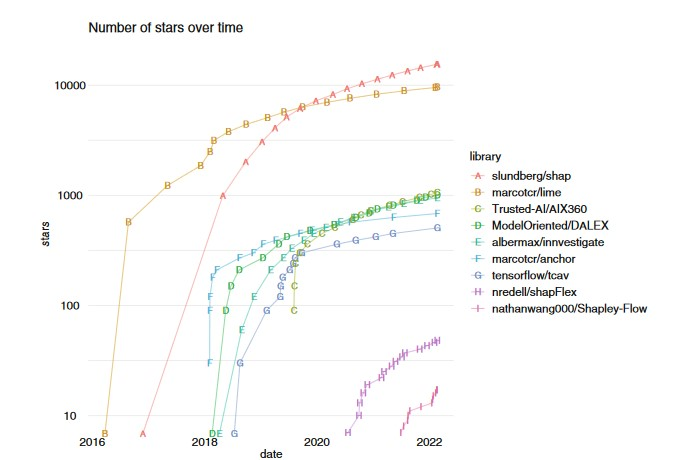
\includegraphics[width=0.8\textwidth]{images/most popular XAI toolboxes - GitHub Stars - xxAI 2022.jpg}
  \caption{The most popular XAI repositories on GitHub (number of stars) as presented in: \cite{holzingerXxAIExplainableAI2022a}.}\label{fig:Popular XAI Tool}
\end{figure}

This methodological approach tackles the delivery of an explanation by weighting each pixel of an input image, producing a visual image of to the end user, with the aim of showing the importance each pixel made to the final classification. This can be problematic, as many of these methods can only highlight the edges of an image, offering little of use in terms of an explanation i.e. the differences between one class and another (\cite{rudinStopExplainingBlack2019}. Saliency maps are also prone to to sensitivities in the data or model, and as such, potentially misleading if used as a sole means of assessment \cite{adebayoSanityChecksSaliency2018a}.

The misleading nature of saliency maps is supported by Kim et al. \cite{kimInterpretabilityFeatureAttribution2018} in an experiment measuring the perceived importance of an image and concept. Participants were shown four images with concept captions (produced using Concept Activation Vectors \cite{kimInterpretabilityFeatureAttribution2018}), each with two corresponding saliency maps (SmoothGrad \cite{smilkovSmoothGradRemovingNoise2017} and Integrated Gradients \cite{adebayoSanityChecksSaliency2018a}) and asked to rate the importance of the image to the model (10-point Likert scale), the importance of the caption (10-point Likert scale), along with their confidence in their answer (5-point Likert scale). The results indicate that due to the percentage of correct answers rated as very confident being equivalent that of incorrect answers, that saliency maps have a tendency to be misleading. There was also a degree of decorrelation in accuracy between the two saliency maps i.e. when one correctly communicated a concept, it was not always true with that of the other. This further supports the notion that post-hoc saliency methods are frequently fragile and limited in their ability to deliver a useful, explanation. This supports the need for inherently interpretable models, of which this research project attempts to tackle.

\subsection{Concept Bottleneck Models}

The emergence and growth in research on Concept Bottleneck Models (CBMs) has been motivated with two key benefits in mind when approaching the task of XAI. Firstly, there is the promise that class classification predictions can be explained using high-level human interpretable concepts produced by a concept predictor \cite{grangeXAISelfexplanatoryAI2022}. Secondly, that a human operator can intervene, altering concept values and monitoring the effect this has on the final prediction \cite{havasiAddressingLeakageConcept2022a}. 

One of the first propositions in this field was that of “Concept Whitening”(CW) \cite{chenConceptWhiteningInterpretable2020}. This purportedly inherently interpretable model, places a bottleneck in a CNN, replacing a batch normalisation (BN) layer with a novel CW layer. By doing so, the latent space of a neural network is “disentangled”, constraining the neurons in the network to realign to the axes of predefined concepts understandable by humans. The research method uses ResNet18, with experiments conducted that assert that the 16th layer provides the clearest approximation of concept alignment. This focus on the penultimate layers of the model, is congruent with the idea that higher-level semantic concepts are present in the latter layers of CNNs (\cite{zhouInterpretingDeepVisual2017}, \cite{grangeXAISelfexplanatoryAI2022}). All experiments using this combination are trained using the Places 365 dataset, with either three or seven simultaneous concepts from the MS COCO dataset.  

It can be argued that the concepts being defined here are quite primitive and limited in dimensionality e.g. “air-plane”, “bed” or “person”, and as such fail to deliver, beyond that of the clarity of a single concept in an image, and is somewhat analogous to a "grandmother cell" in neuroscience. It therefore falls short of denoting the deeper semantic descriptors of an images features e.g. if the image is that of an  air-plane, why is it so? Presence of wings, flying in the sky, shape etc. Rather the output focuses on what it is not e.g. an air-plane is not a table, bed or boat. This is a clear limitation of the training data used (Places 365 \& MS COCO), of which is such granular details are not inclusive. Consequently, the paper concludes, that if a full explanation on each computation were to be delivered then this would lead to a restriction on flexibility, however one may determine that the complexity would be considerably reduced if only applied within an a single expert domain. The transference of the CW model to an expert domain is attempted, focusing on skin lesions, however it is limited by the use of only two concepts, age and legion size, of which age is discovered to play no importance to classification. Opposingly, the size of the legion (>=10) is in the third quartile of importance (of 512 axes), a concept that is know to be used by physicians for diagnosis of skin lesions \cite{walterUsing7pointChecklist2013}. This brief insight into the importance of expert domain knowledge reinforces the need for the incorporation of well defined concepts based upon existing empirical evidence, reinforcing the body research undertaken in this project.

The pursuit of a delivering a comprehensive explanation has led to the prolific development of new concept bottleneck models (CBM), both ante and post-hoc (\cite{kohConceptBottleneckModels2020}, \cite{margeloiuConceptBottleneckModels2021}, \cite{havasiAddressingLeakageConcept2022a}, \cite{yuksekgonulPosthocConceptBottleneck2022}). 

Koh et al. \cite{kohConceptBottleneckModels2020} offer three CBM models for exploration: 
(1)	Independent bottlenecks, whereby concepts and classification are learnt in separate algorithms, with the resultant learnt concepts used for classification at test time.
(2)	Sequential bottlenecks, whereby the concept is learnt, with the learnt concepts used to inform classification learning.
(3)	Joint bottlenecks, whereby the concept and classification are both learnt in combination during training, whereby $\lambda$ regularisation factor is adjusted using the combined losses  

The findings illuminate that not only by using human annotated data for training, but along with the intervention by an expert (particularly independent bottlenecks), a model can be updated if an artefact is incorrectly identified as a concept/feature, substantially improving accuracy beyond that of a standard model, with an overall observation that there is not in fact a trade-off between high task accuracy and high concept accuracy \cite{kohConceptBottleneckModels2020}.

Due to the improved levels of predictive performance (analysis of Root Mean Squared Error - RMSE) through concept refinement, Koh et al. take preference to the proposed joint CBM model. Yet it is noted that the benefits of intervenability in joint models is detrimental to performance. To the contrary, independent models benefited the most from expert intervention of concept prediction using ground truths.

The quality of the output of all three models proposed by Koh et al. is interrogated by Margeloiu et al.'s \cite{margeloiuConceptBottleneckModels2021} three desiderata of a CBM:
1.	Interpretability: Being able to note which concepts are important for the targets. 
2.	Predictability: Being able to predict the targets from the concepts alone. 
3.	Intervenability: Being able to replace predicted concept values with ground truth values to improve predictive performance.

The methodology used by Margeloiu et al. to critique Koh et al.’s three CBM models, requires the development of a concept oracle model (CO); a model using ground truths to predict target images. The CO is used to compare through the correlation of the root mean square error (RMSE) of each CMB model and CO. The finding suggests that independent CMBs and COs have a far higher coefficient of determination. This observation aligns with the hypothesis that predicted concepts (as per sequential and joint CBMs) are not used as intended, but rather as proxies to incorporate target information, shown with a vastly reduced RMSE as the level of concept intervention increases, particularly that of independent CBMs (see Fig 4 in \cite{kohConceptBottleneckModels2020}). It is suggested by Margeloiu et al. that one of the reasons for low correlation of concepts in sequential and joint CBMs to COs is a result of the use of one-hot encoding for concept values i.e. concepts are binary (0 or 1). Leading on to suggestions of further study, through the analysis of the variability of concept representations by means of binary and scalar concepts, and one-hot encoded categoricals. It should be noted that some analysis of binary and scalar concepts is tackled later on within this research project manuscript. Margeloiu et al. also take on the use of saliency maps (Integrated Gradients with Gaussian Noise baseline) to try and assess the predicted concepts visually, showing attention across the whole image rather than that of the defined feature, however, as commented by many others, saliency maps are unable to map concepts in any meaningful manner (\cite{rudinStopExplainingBlack2019}, \cite{adebayoSanityChecksSaliency2018a},\cite{kimInterpretabilityFeatureAttribution2018}).

\subsection{Post-hoc Concept Bottleneck Models}

Complementary to the development of CMBs, much research has been undertaken in the development of post-hoc CBM (PCBM) methods (\cite{havasiAddressingLeakageConcept2022a}, \cite{yuksekgonulPosthocConceptBottleneck2022}, \cite{daneshjouSkinConSkinDisease2022}), of which attempt to address multiple issues, such as the loss of concept clarity or “leakage” \cite{mahinpeiPromisesPitfallsBlackBox2021}. It is speculated that the cause of leakage may be the result of an overlap of concepts in the concept predictor layer due an insufficient concept set being available e.g. some classifications may require more concepts than others, or that “soft” concepts i.e. non-binary concepts (probabilities, often between 0 and 1) allow unintended information to be conveyed. In conclusion, resultant leakage muddies both interpretability and the ability to effectively intervene on the concept predictor. The alternative to soft CBMs is that of hard CBMs, whereby concepts are binary. One may consider this approach to be more truthful, as leakage between concepts is prevented, yet this method is prone to lower classification accuracy unless all concept details are captured correctly. There is no flexibility for the system to leak knowledge into another concept, thus  thorough domain knowledge is required to prevent miscoding concepts, either by not getting the quantity correct, through human error in labelling the training data, or a mutual lack of understanding between the user, the domain, the input, and the models deliverables (perhaps there is hidden knowledge the model requires that is not innately intelligible by humans). This notion is contrary to the supposition by Margeloiu et al. that hard CBMs may be responsible for the low correlation of concepts in sequential and joint CBMs. 
A conclusion may be drawn that naturally, some concept features could always be considered binary due to their intrinsic nature e.g. obsidian rocks will always have a glass like texture, or marble being composed of crystals. However, it is less clear if the network would benefit from further granularity, i.e. how much of said concept is present in the image used for training.

Havasi et al. \cite{havasiAddressingLeakageConcept2022a} propose two further means of addressing leakage and improving performance of hard concept CBMs: (1) a side channel model and (2) an auto-regressive architecture. Prior to using either tools a model is first analysed to see if the concepts are sufficient in predicting the final label classification, or if more information is desired – the lack of a Markovian assumption. The side channel model is a small single layer which is trained concurrently with the hard CBM from a set of latent concepts, with the flexibility to infer how many concepts are required for label prediction. This side-channel enables one to estimate the completeness of the original concepts, and therefore can be used as a form of diagnosis to infer if there are key concepts missing. Yet, on closer inspection it is clear that much of the side channel information has the propensity to deliver concepts uninterpretable by humans – something that may or not be desirable depending upon the domain and accuracy required by the end user. The second tool is that of an auto-regressive architecture that allows for hard CBMs to learn correlations between concepts, therefore re-weighting concepts, with interventions also affecting concept predictions of prior concepts. They note that normalisation is of upmost importance to ensure that correct predictive distribution. Both methods come at the cost of increased  computation; however they do put hard CBMs at an accuracy level equivalent to that of soft CBMs. This may be desirable in some domains whereby concept knowledge is always translatable in a binary manner, however in many domains this is not always the case, and if applied then the initial mandate, to enable human interpretability, is lost.

A novel post-hoc CBM (PCBM) model is proposed by Yuksekgonul et al. \cite{yuksekgonulPosthocConceptBottleneck2022}, attempting to tackle three key limitations of CBMs: access to data i.e. the laborious task of annotating or collating a concept dataset, increasing performance, and the enablement of intervention by human input. The first task of collating a concept databank is approached in two ways, through utilising Concept Activation Vectors (CAVs) or with state of the art (SOTA) multi-modal models such as "Contrastive Language Image Pre-Training" (CLIP) \cite{radfordLearningTransferableVisual2021}. 
The use of a CAV is utilised by learning concepts selected by a domain expert, or automatically from the data, that positively or negatively associate with the image. This method is pragmatic in that it does not require the training data to mirror the data used to train the backbone model, as per requirement of a CBM. A linear standard vector model (SVM) is then used to learn the corresponding CAV, using the positive and negative examples to denote the vector notal to the linear classification boundary.

The second method for constructing a concept bank is through the utilisation of the text encoder from the multi-modal model CLIP, of which contains both text and image encoders to map a description to a shared embedding space. A concept description vector is obtained through collating the relevant text embeddings to be utilised in combination with an open knowledge graph, ConceptNet \cite{speerConceptNetOpenMultilingual2017}, to collate the relationships between classes and concepts. 

Once a concept subspace is learnt through either CAV or CLIP, a sparse linear model or decision tree is used for prediction due to the inherent clarity and insight with which one can observe a decision being made. It is noted that the richness of the concept subspace is important to the performance accuracy of the PCBM, of which would no doubt disincentivise any potential user for uptake over that of a normal model. An attempt to solve this issue is made by utilising a sequential residual predictor, that attempts to retain some of the original model’s accuracy, a concept denoted as Hybrid Post-hoc CBMs (PCBM-h). Despite this effort to debug the CBM model, there is still the  risk that one may be limited with a poor concept library, ill equipped to express and solve the task it is required, and potentially containing and reinforcing biases. Despite this, Daneshjou et al. \cite{daneshjouSkinConSkinDisease2022} successfully incorporates the PCBM methodology into a novel work flow, using expert dermatologist defined concepts to develop SkinCon. A dataset of existing image annotations was used, and clarified using expert intervention..

Others have approached the matter of concept completeness/sufficiency and discovery in alternative means, such as ConceptSHAP \cite{yehCompletenessawareConceptBasedExplanations2019}. Yeh et al.’s method delivers a completeness score, shedding light on how sufficient concepts are for delivering an explanation, along with a means of to alight how important each concept is to an input by adapting the widely used Shapley value method \cite{shapley17ValueNPerson1953}. The method uses concepts that are common across all classes as opposed to one, postulating that shared class concepts are useful for interpretation of the model, e.g. one may determine through analysis of the concepts by nearest neighbour, that the shape of an animal’s head is important and shared between multiple classes. In an expert domain, the idea of shared concepts is often common place due to the scope being local rather than global. A quick alternative to this method, often used, is to calculate the L2 norm of a the weights in a model to deride which features are most important. However, unlike Shapley values, L2 norm cannot capture the nuanced interaction between individual features in the same way. As such, the incorporation of ConceptSHAP into the realm of CBMs is arguably a vital addition to the AI and ML practitioners toolbox.

\subsection{Concept Bottleneck Models and Large Language Models}

SOTA CBMs have begun leveraging the use of Large Language Models (LLMs), such as aiding with the laborious task of annotating data sets. Language Guided Bottlenecks (LaBo) \cite{yangLanguageBottleLanguage2023}, does so by aligning GPT-3's sentence based concepts using CLIP to form a bottleneck layer. There are some limitations, such as fine tuning the output of GPT-3, restricting the sentence length, and preventing the use of class names. Yet this is arguably preferable as the generated concepts can be controlled and chosen based upon a number of factors, such as interpretabilty, classification accuracy, and those which are highly discriminative and recognisable by CLIP. As such, this model strongly leans towards the the classification of being ante-hoc/inherently interpretable, as it essentially focuses on the fine tuning of CLIP. However the performance is restricted by the training data of GPT-3 (at least in this iteration), which excels in common categories, yet rapidly falls short with delivering higher granularity in more nuanced fields of enquiry, reducing it's potential use case for a number of expert domains. The concept of integrating LLMs, despite being out of the remit of this project, is one of significant future interest, particularly with the development of new LLMs that can be fine tuned to focus on specific expert domains. Yet, as previously noted, LLMs are vastly more difficult to explain in comparison to current NN methods, requiring whole new methodologies in the realm of XAI \cite{zhaoExplainabilityLargeLanguage2023}.  

Other developments incorporating LLMs explore the incorporation of multiple models and multiple input modalities e.g. ChatCAD \cite{wangChatCADInteractiveComputerAided2023} for medical image diagnosis. ChatCAD leverages multiple SOTA computer aided diagnosis (CAD) networks e.g. a disease classifier, lesion segmentor, and report generator, from which a combined prompt text can be generated for input into an LLM such as ChatGPT. In doing so a condensed report of the diagnosis is produced, leveraging the the models knowledge of the medical field \cite{gilsonHowDoesChatGPT2023}, and enabling the user to interrogate the report through conversational enquiry. 

Zhang et al. \cite{zhangMayAskFollowup2023} support the notion of free-form conversation with a network, demonstrating that comprehension, acceptance, trust and collaboration are significantly improved between the user and AI model. However their experiment is not without limitations, such as the use of the wizard-of-oz methodology and only two two feature attribution tools (LIME and Grad-CAM) being used as a means of explanation (the limitations of which have previously been stated).

Further developments in multi-modal LLMs such as NExT-GPT \cite{wuNExTGPTAnytoAnyMultimodal2023} indicate the possibility to deliver upon potentially higher levels of explainability as well as inclusivity via the use of modality switching e.g. from natural language text, to image, video or audio, subsequently delivering a more human like means of interaction. NExT-GPT does so by the use of modality-switching instruction tuning (MosIT), in combination with a manually curated high quality dataset. Despite the impressive possibilities of this model (requiring only 1\% of the parameters to be updated during training for each new modality), with hopes of incorporating additional modalities in its next iteration e.g such as tables, figures, heat maps and so on; the manual curation of a bespoke dataset (MosIT) is somewhat concerning. As with all data sets, there is always the risk of human bias being encoded, unconsciously or otherwise, through the selection of data and its subsequent annotations. This further highlights the need for legislation and the regulation of data used to train such models. 

With the ever increasing complexity of AI systems that combine multiple models and modalities (\cite{wangChatCADInteractiveComputerAided2023}, \cite{wuNExTGPTAnytoAnyMultimodal2023},\cite{yangLanguageBottleLanguage2023}), it will become an ever increasing challenge to incorporate explainability and interpretabilty throughout. Therefore, the use of accurate, explainable, and interpretable CBMs hold a strong defence to be included as an essential item in a developers toolbox when delivering a trustworthy complex AI system, offering a glimmer of transparency, in light of other elements which may appear opaque.